\setchapterpreamble[o]{
	\vspace*{-2.60cm}\hspace*{-2.25cm}
	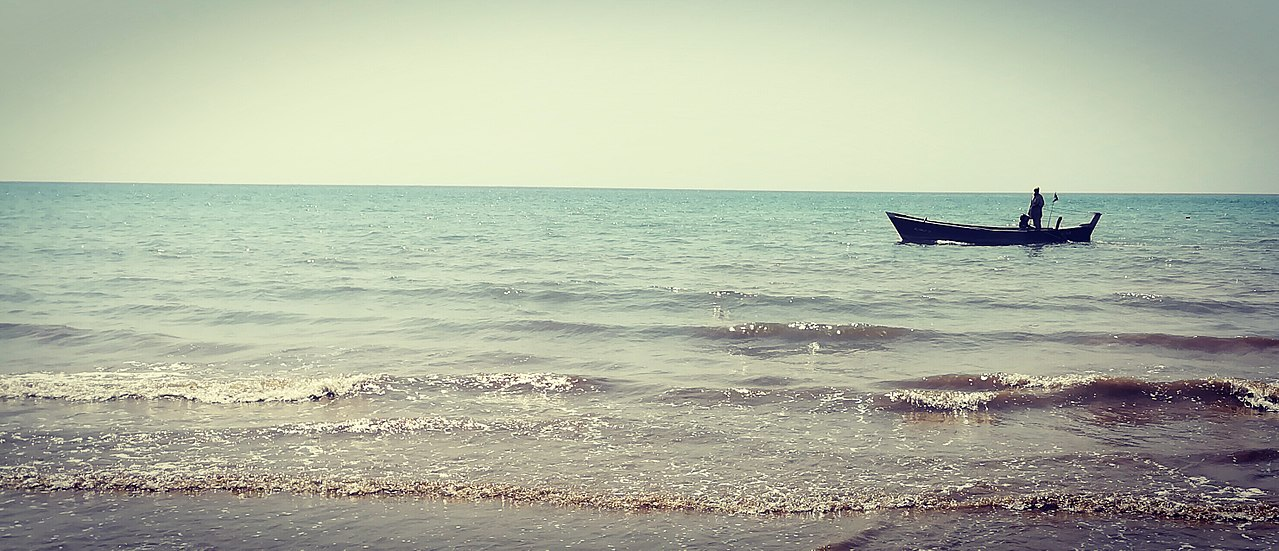
\includegraphics[width=\paperwidth,height=8cm,keepaspectratio=false]{images/seaside}
	\captionsetup{type=figure}
	\caption[seaside]{By Bushra Feroz - Own work, CC BY-SA 4.0, 
\url{https://commons.wikimedia.org/w/index.php?curid=68724647}}
}
% beforeskip=-(figure_height-top_margin)
\RedeclareSectionCommand[beforeskip=-5.40cm]{chapter}
\setchapterpreamble[u]{\margintoc}
\chapter{Figures and Tables}
\RedeclareSectionCommand[beforeskip=0cm]{chapter}

\section{Normal figures and tables}

%\marginnote{\blindtext}

\blindtext

\begin{figure}[h]
	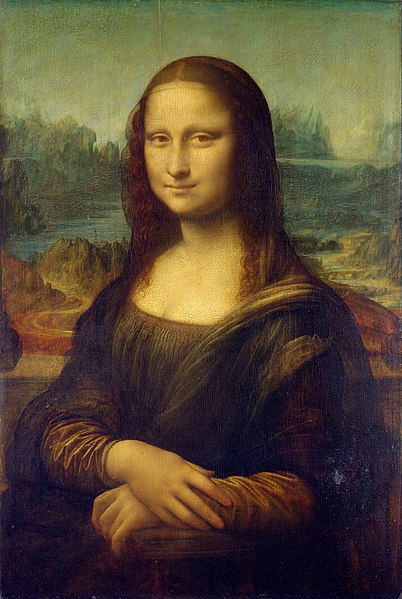
\includegraphics[width=0.4\textwidth]{monalisa}
	\caption{It's Mona Lisa again. \blindtext}
\end{figure}

\blindtext

\begin{table}
\begin{tabular}{ |c|c|c|c| } 
\hline
col1 & col2 & col3 \\
\hline
\multirow{3}{4em}{Multiple row} & cell2 & cell3 \\ 
& cell5 & cell6 \\ 
& cell8 & cell9 \\ 
\hline
\end{tabular}
\caption{A useless table. \blindtext}
\end{table}

\blindtext

\section{Margin figures and tables}

\blindtext

\begin{margintable}[*-6]
\begin{tabular}{ |c|c|c|c| } 
\hline
col1 & col2 & col3 \\
\hline
\multirow{3}{4em}{Multiple row} & cell2 & cell3 \\ 
& cell5 & cell6 \\ 
& cell8 & cell9 \\ 
\hline
\end{tabular}
\caption{A useless table.}
\end{margintable}

\section{Wide figures and tables}
